\chapter{Problem Analysis}
\label{cha:Problem Analysis}

\section{Lane Merging Problems}
\label{sec:Lane Merging Problems}
Vehicles may have to merge into another lane for a number of reasons. In this paper we focus on merges made at 'critical positions' such as junctions. This analysis could later be applied to merges made at non-critical points, though centralised approaches may struggle here.

\subsection{Single-to-Single Merge}
\label{subsec:Single-to-Single Merge}
A single-to-single merge (S2S merge) describes a situation where a vehicle moves from a single lane road into another single lane road, as seen in Figure \ref{fig:S2SMerge}. In this situation we label the lane that vehicles are moving from the 'current lane', and we label the lane that vehicles move to the 'target lane'. We describe the vehicles that start on the current lane as 'merging vehicles' and the vehicles that start on the target lane as 'target vehicles'. We have one critical position where the current lane meets the target lane.

\begin{figure}[htb]
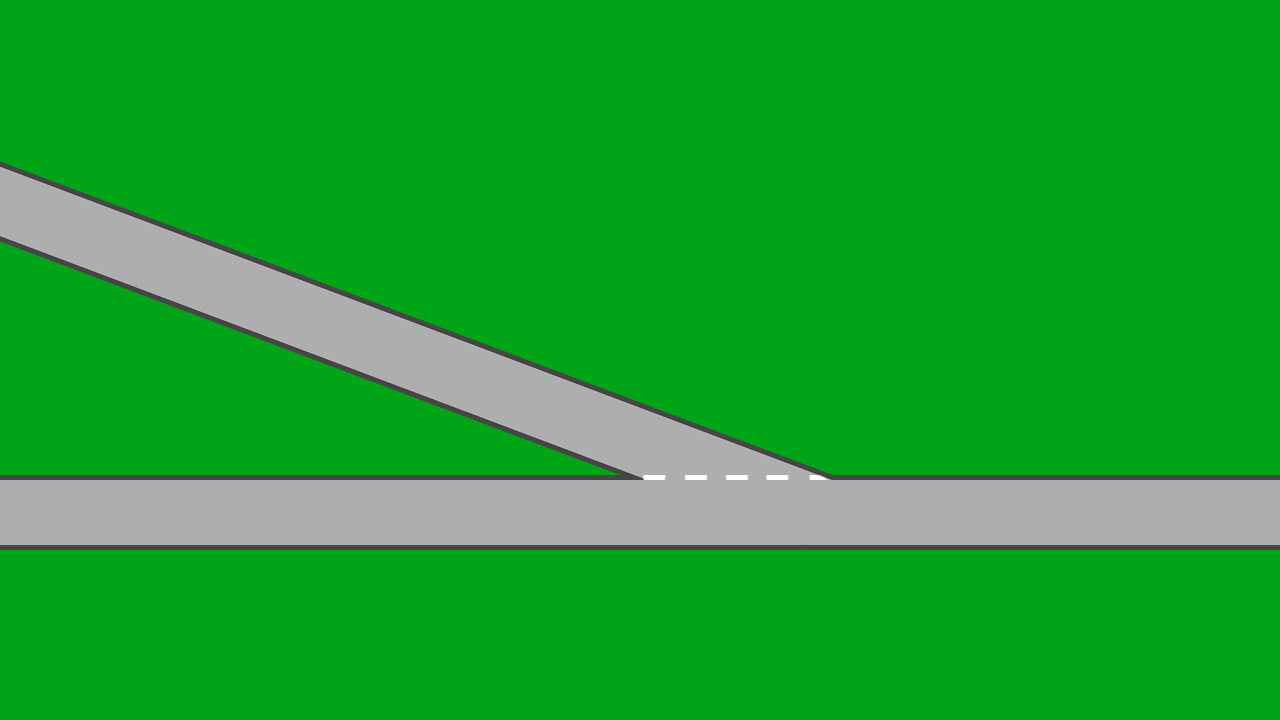
\includegraphics[width=\textwidth]{lane_diagrams/s2s.png}
\caption{A road with a single-to-single lane merge (S2S)}
\label{fig:S2SMerge}
\end{figure}

\newtext{New text below}

The main issue with an S2S merge stems from the limited options available to vehicles arriving at the critical position. Target vehicles do not have the opportunity to move laterally out of the way of merging vehicles, and vehicles on both lanes could struggle to reduce their velocity without affecting their successors. A solution to an S2S merge would have to satisfy the following conditions:

\begin{enumerate}
\item \textit{No collisions}
This means avoiding collisions at the critical position between merging vehicles and target vehicles, as well as avoiding collisions between vehicles on the same lane.
\item \textit{Minimise delays to both lanes}


\end{enumerate}

\subsection{Single-to-Double Merge}
\label{subsec:Single-to-Double Merge}

\begin{figure}[htb]
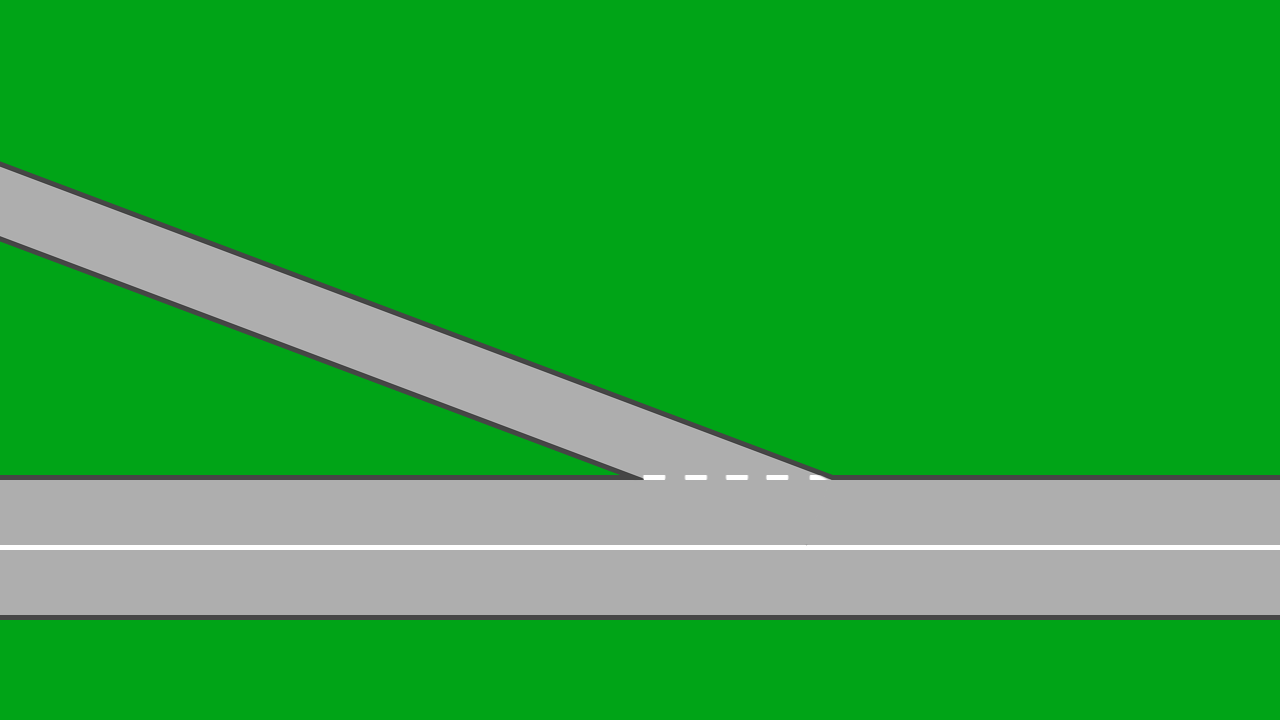
\includegraphics[width=\textwidth]{lane_diagrams/s2d.png}
\caption{A road with a single-to-double lane merge (S2D)}
\label{fig:S2DMerge}
\end{figure}


\subsection{Double-to-Double Merge}
\label{subsec:Double-to-Double Merge}

\begin{figure}[htb]
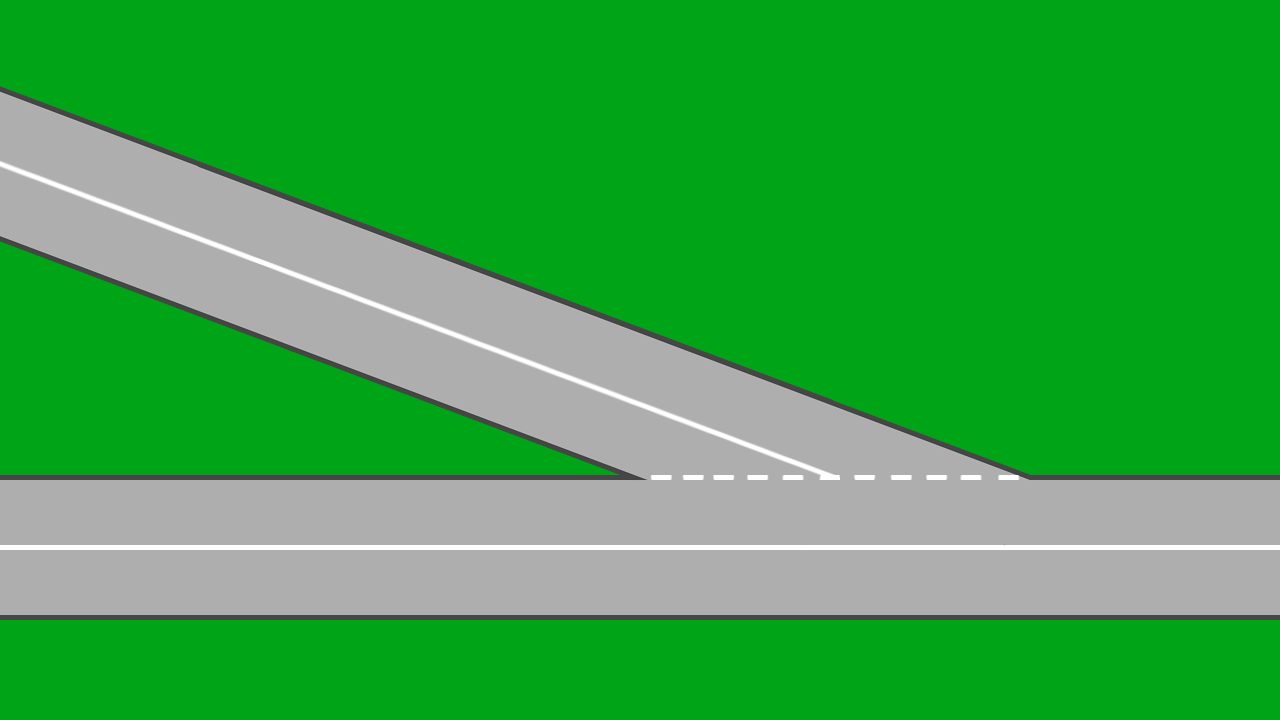
\includegraphics[width=\textwidth]{lane_diagrams/d2d.png}
\caption{A road with a double-to-double lane merge (D2D)}
\label{fig:D2DMerge}
\end{figure}

\subsection{Lane Obstruction Merge}
\label{subsec:Lane Obstruction Merge}

\begin{figure}[htb]
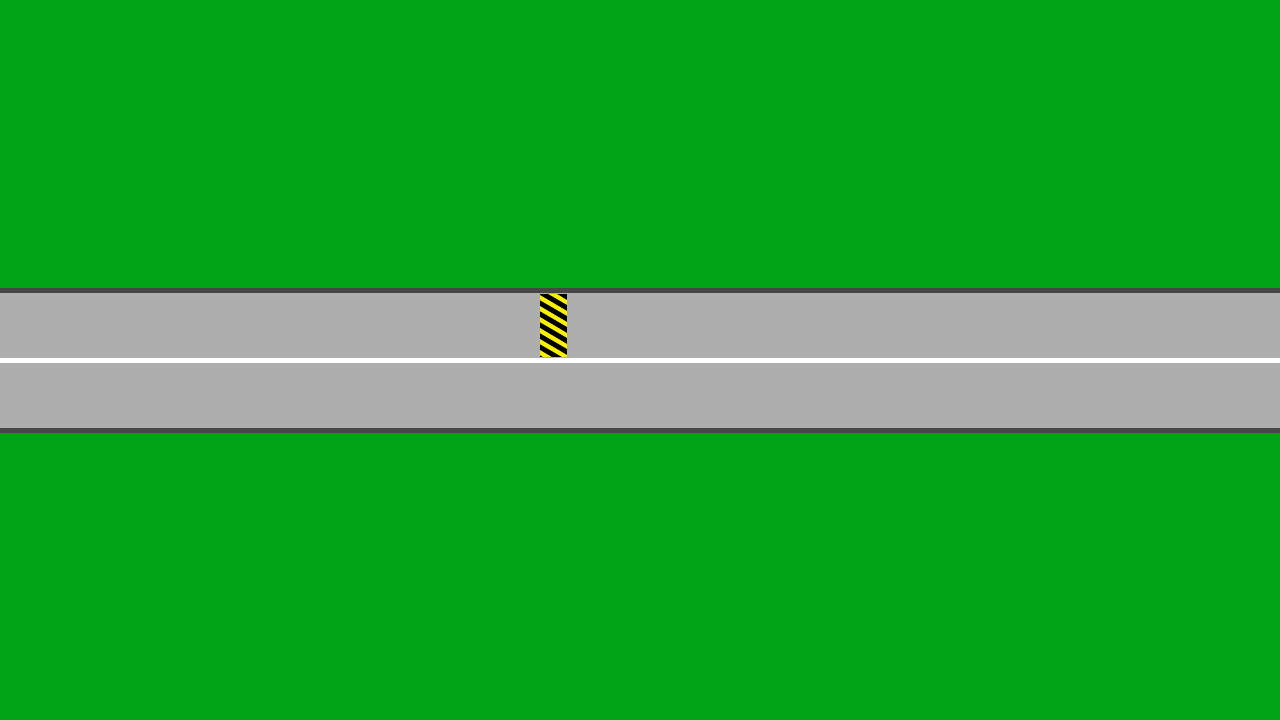
\includegraphics[width=\textwidth]{lane_diagrams/lane_blocker.png}
\caption{A road with a lane obstruction}
\label{fig:LaneObstruction}
\end{figure}

\section{Measuring Success}
\label{sec:Measuring Success}
In order to evaluate the effectiveness of solutions to the problems we need to define measurements of success. Above we defined conditions that must be satisfied for a solution to be acceptable. Here we discuss how to measure how well a solution meets these conditions.

\subsection{Throughput}
\label{subsec:Throughput}

\subsection{Delay}
\label{subsec:Delay}

\subsubsection{Average Delay}
\label{subsubsec:Average Delay}

\subsubsection{Worst Delay}
\label{subsubsec:Average Delay}

\subsection{Traffic Density}
\label{subsec:Traffic Density}